\chapter{Plan de Capacitación, Implantación y Puesta en Marcha}

\subsection{Estado del Proyecto}
Actualmente, el proyecto se encuentra finalizado. Esto quiere decir que todos los módulos, requerimientos funcionales y objetivos propuestos han sido alcanzados con éxito.

Si bien el software del proyecto está completamente finalizado, éste aún no pasa a ser utilizado por el público, por lo que sigue estando en una etapa de puesta en marcha cerrada sólo para la administración y miembros del staff de RVA.

\subsection{Implantación y Puesta en Marcha}
Como se mencionó anteriormente en el estado del proyecto, la implantación del software está tomando una ruta gradual, en la que primero se le ha permitido sólo al staff de RVA interactuar con la aplicación web para que puedan familiarizarse con el nuevo sistema.

Eventualmente, para la puesta en marcha oficial, la página será lanzada para el público general.

\subsection{Plan de Capacitación}
Para este proyecto, se ha considerado un plan de capacitación que consiste en un video explicativo simple \cite{adminwalkthrough}, en el cual se indica como utilizar la plataforma en tiempo real, entrando en detalle en cada una de las funcionalidades relevantes del software. La \autoref{fig:training} es una captura del video que fue subido a la plataforma de YouTube.

\begin{figure}[H]
  \begin{center}
    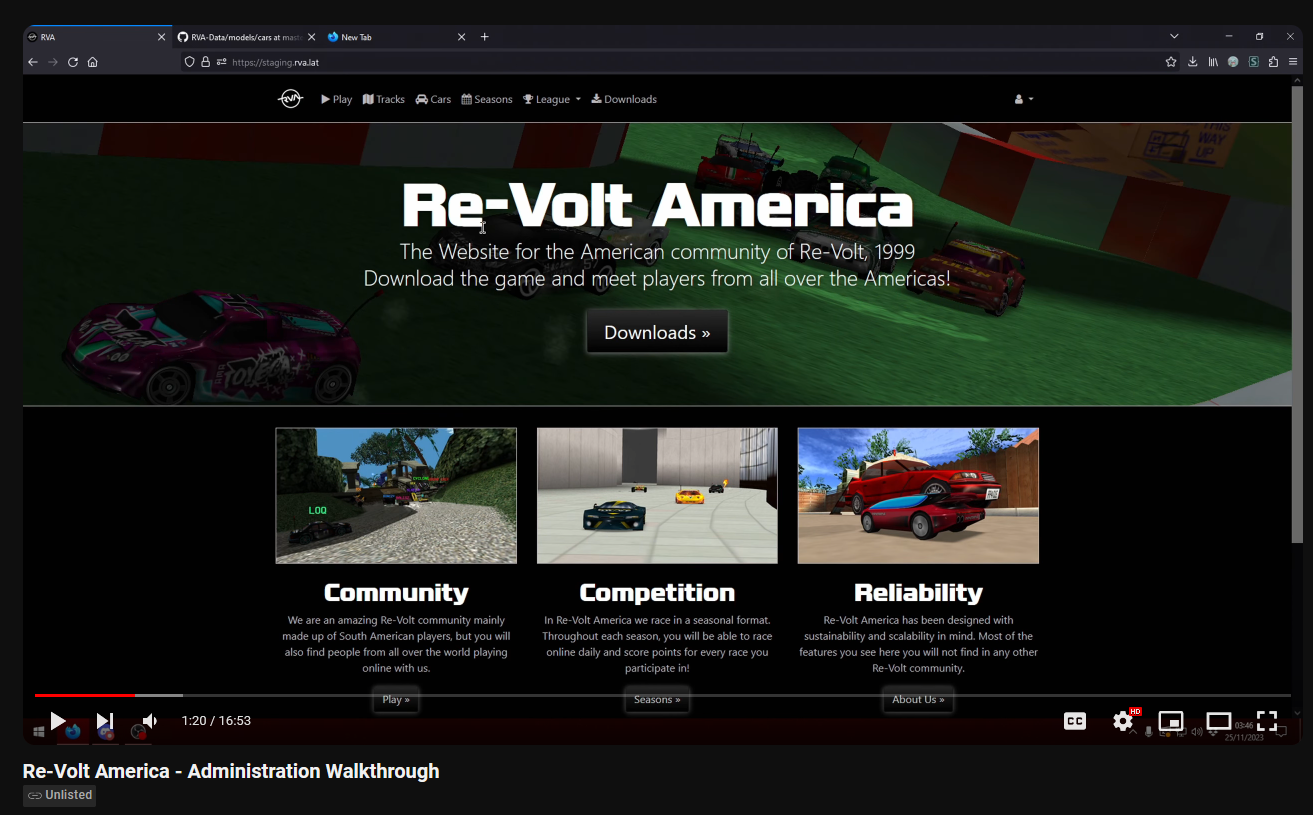
\includegraphics[width=15cm, height=9cm]{training.png}
  \end{center}
  \caption[Video de capacitación para administradores]{Video de capacitación para administradores}
  \label{fig:training}
\end{figure}
